\documentclass[10pt,a4paper]{article}
\usepackage[utf8]{inputenc}
\usepackage{amsmath}
\usepackage{amsfonts}
\usepackage{amssymb}
\usepackage{graphicx}
\usepackage{verbatim}
\usepackage[margin=1in]{geometry}

\setlength\parindent{0pt} % Removes all indentation from paragraphs

\author{Nikola Janju\v{s}evi\'{c}}
\title{ECE471, Selected Topics in Machine Learning \\ Assignment 2}
\date{September 11, 2018}

\begin{document}
\begin{large}
ECE471, Selected Topics in Machine Learning -- Assignment 2 \\
\end{large}
Convolution Neural Net MNIST Classifier \\
Nikola Janju\v{s}evi\'{c} \\
September 11th 2018 
 
\begin{verbatim}
# Nikola Janjusevic
import matplotlib.pyplot as plt
import tensorflow as tf
import numpy as np
import time
from tqdm import tqdm
from numpy.random import *

logs_path = "./tf_logs/"

# hyper-parameters
dim_layer1 = 16
dim_layer2 = 32
num_classes = 10
NUM_BATCHES = 200
BATCH_SIZE = 500
NUM_EPOCHS = 8 # not technically using epochs but im keeping it.
learning_rate = 0.01
display_epoch = 1

# convolution layer parameters
k1 = 5
pool1 = 2
k_stride1 = 2
p_stride1 = 2

# regularization parameters
l2_lambda = .01/(k1*k1*dim_layer1 + dim_layer1*dim_layer2)
drop_out = .9

# https://stackoverflow.com/questions/38592324/one-hot-encoding-using-numpy/38592416
def get_one_hot(targets, nb_classes):
    res = np.eye(nb_classes)[np.array(targets).reshape(-1)]
    return res.reshape(list(targets.shape)+[nb_classes])

class Data(object):
    def __init__(self):
        mnist = tf.keras.datasets.mnist
        # 60k training, 10k testing
        (x_train, y_train),(x_test, y_test) \
            = mnist.load_data()
        # normalize [0, 255] to [0,1]
        self.x_train = x_train.reshape(x_train.shape[0],28,28,1) / 255.0
        x_test  = x_test.reshape(x_test.shape[0],28,28,1) / 255.0
        [self.x_val, self.x_test] = np.split(x_test,2)
        # digits [0,9] to length 10 one_hot vectors
        self.y_train = get_one_hot(y_train, num_classes)
        y_test = get_one_hot(y_test, num_classes)
        [self.y_val, self.y_test] = np.split(y_test,2)

        self.index_train = np.arange(x_train.shape[0])
        self.index_test = np.arange(x_test.shape[0])

    def get_batch(self):
        choices = choice(self.index_train, size=BATCH_SIZE)
        return self.x_train[choices,:,:,:], self.y_train[choices,:]

# convolution layer: conv-> +bias -> activation -> pool
def conv_layer(input, W, b, k_stride=1, pool=2, p_stride=2):
    x = tf.nn.conv2d(input, W, strides=[1, k_stride, k_stride, 1], padding="VALID")
    x = tf.add(x,b)
    x = tf.nn.relu6(x)
    return tf.nn.avg_pool(x, ksize = [1, pool, pool, 1],
        strides = [1, p_stride, p_stride, 1], padding="VALID")

# fully connected layer
def fc_layer(input, W, b):
    x = tf.add( tf.matmul( tf.reshape(input, [-1, tf.shape(W)[0]]), W ), b)
    return tf.nn.relu6(x)

x = tf.placeholder(tf.float32, [None,28,28,1])
y = tf.placeholder(tf.float32, [None,10])
keep_prob = tf.placeholder(tf.float32) # for dropout

# f:R28x28 -> R10
def f(x):
    layer_1 = tf.nn.dropout(
        conv_layer(x, weights['w1'], biases['b1'], k_stride=k_stride1,
            pool=pool1, p_stride=p_stride1),
        keep_prob
    )
    layer_2 = tf.nn.dropout(
        fc_layer(layer_1, weights['w2'], biases['b2']),
        keep_prob
    )
    return tf.squeeze(
        tf.add( tf.matmul(layer_2, weights['out']), biases['out'] )
    )

# width/height dimension after conv
d1 = int( np.ceil(float(28 - k1 + 1) / float(k_stride1) ) )
# width/height dimension after pooling
dp1 = int( np.ceil(float(d1 - pool1 + 1) / float(p_stride1) ) )

# Store layers weight & bias
# default dtype=float32
weights = {
    'w1': tf.Variable(tf.random_normal([k1,k1,1,dim_layer1])), # kernel
    'w2': tf.Variable(tf.random_normal([dp1*dp1*dim_layer1,dim_layer2])),
    'out': tf.Variable(tf.random_normal([dim_layer2, num_classes]))
}
biases = {
    'b1': tf.Variable(tf.random_normal([dim_layer1])),
    'b2': tf.Variable(tf.random_normal([dim_layer2])),
    'out': tf.Variable(tf.random_normal([num_classes]))
}

# models
logits = f(x)
prediction = tf.nn.softmax(logits)

correct_pred = tf.equal(tf.argmax(prediction, 1), tf.argmax(y, 1))
accuracy = tf.reduce_mean(tf.cast(correct_pred, tf.float32))

# binar cross entropy loss with L2 penalty on weights
loss = tf.reduce_mean( tf.losses.softmax_cross_entropy(y, logits) ) + \
    l2_lambda*tf.reduce_sum(
        [tf.nn.l2_loss(var) for var in
        tf.get_collection(tf.GraphKeys.TRAINABLE_VARIABLES)]
    )
optim = tf.train.AdamOptimizer(learning_rate=learning_rate).minimize(loss)
init = tf.global_variables_initializer()

# Create a summary to monitor cost tensor
tf.summary.scalar("loss", loss)
# Create a summary to monitor accuracy tensor
tf.summary.scalar("accuracy", accuracy)
# Merge all summaries into a single op
merged_summary_op = tf.summary.merge_all()

with tf.Session() as sess:
    data = Data()
    sess.run(init)
    # op to write logs to Tensorboard
    summary_writer = tf.summary.FileWriter(logs_path,
        graph=tf.get_default_graph())
    # training
    for epoch in range(NUM_EPOCHS):
        avg_cost = 0.
        num_batches = NUM_BATCHES
        for i in tqdm(range(num_batches)):
            xb, yb = data.get_batch()
            loss_np, _, summary = sess.run([loss, optim, merged_summary_op],
                feed_dict={x: xb, y: yb, keep_prob: drop_out})
            # logs every batch
            summary_writer.add_summary(summary, epoch * num_batches + i)
            avg_cost  += loss_np/num_batches
        # Display logs per epoch step
        if (epoch+1) % display_epoch == 0:
            print("Epoch:", '%02d' % (epoch+1),
                "cost=", "{:.6f}".format(avg_cost))
        print('Validation Set Accuracy:',
            accuracy.eval({x: data.x_val, y: data.y_val, keep_prob: 1.0}))

    # Test the model on separate data
    print('Test Set Accuracy:',
        accuracy.eval({x: data.x_test, y: data.y_test, keep_prob: 1.0}))

    print("Run the command line:\n--> tensorboard --logdir=./tf_logs ")
\end{verbatim}

\begin{figure}[h]
\centering
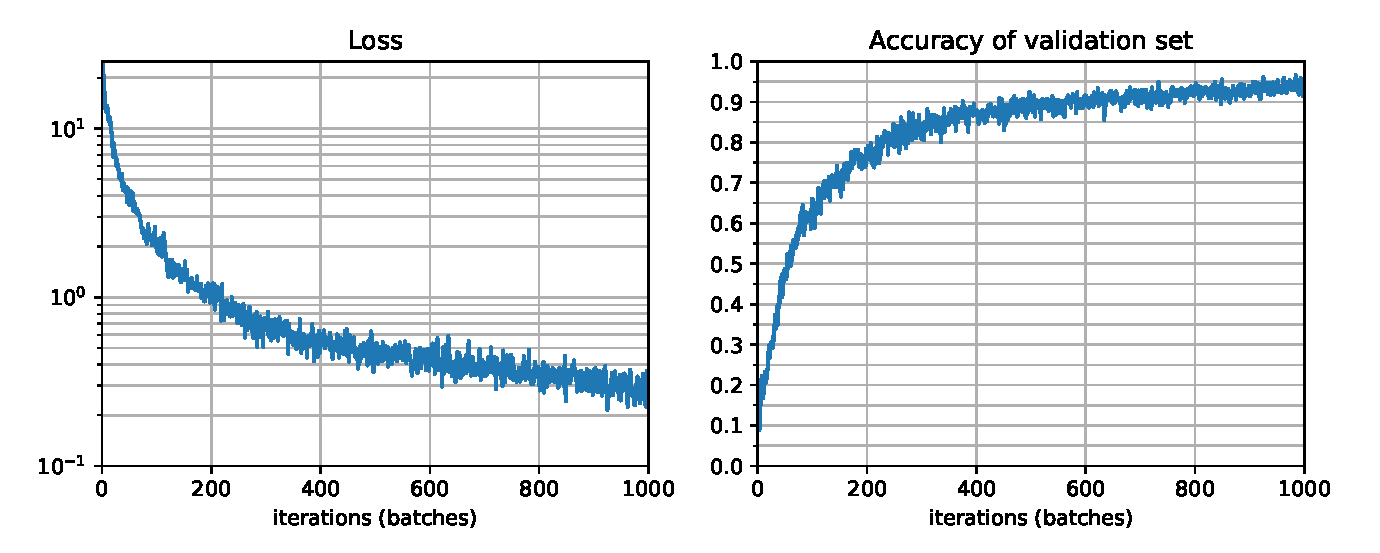
\includegraphics[width=\textwidth]{Figure_1.pdf}
\caption{CNN performance with the hyper parameters specified at the top of the program achieving. \%98.14 accuracy on the test set}
\end{figure}

\end{document}